\documentclass{article}

% Language setting
% Replace `english' with e.g. `spanish' to change the document language
\usepackage{biblatex} %Imports biblatex package
\addbibresource{sample.bib}
\usepackage[english]{babel}
\usepackage{array}
\usepackage{amsmath}
\usepackage{pythonhighlight}
\newcolumntype{P}[1]{>{\centering\arraybackslash}p{#1}}
\newcolumntype{M}[1]{>{\centering\arraybackslash}m{#1}}

% Set page size and margins
% Replace `letterpaper' with `a4paper' for UK/EU standard size
\usepackage[letterpaper,top=2cm,bottom=2cm,left=3cm,right=3cm,marginparwidth=1.75cm]{geometry}

\usepackage{amsmath}
\usepackage{graphicx}
\usepackage[colorlinks=true, allcolors=blue]{hyperref}
\usepackage{setspace}
\usepackage{booktabs}
\usepackage[T1]{fontenc}
\usepackage{longtable}
\doublespacing

\begin{document}
\begin{titlepage}

\centering
\scshape
\vspace{\baselineskip}

%
\rule{\textwidth}{1.6pt}\vspace*{-\baselineskip}\vspace*{2pt}
\rule{\textwidth}{0.4pt}

{\Huge \textbf{\textsc{NPRE 449: Homework 3 \\
\vspace{15pt}}}}

\rule{\textwidth}{0.4pt}\vspace*{-\baselineskip}\vspace{3.2pt}
\rule{\textwidth}{1.6pt}\vspace{6pt}
%%\centerline{\textit{University of Illinois at Urbana-Champaign}} 
\vspace{1.5\baselineskip}


\large \centerline{\textbf{Author:} Nathan Glaser}
\large \centerline{\textbf{Net-ID:} nglaser3}
\quad

\vfill
\large \centerline{September 18, 2024}
%
\pagenumbering{gobble}
\end{titlepage}

\tableofcontents
\newpage
\pagenumbering{arabic}

\section*{Question 1}
\addcontentsline{toc}{section}{\protect\numberline{}Question 1}

To begin, the system analyzed in this question is presented in Fig. \ref{fig:q1_config}.
\begin{figure}[!h!]
    \centering
    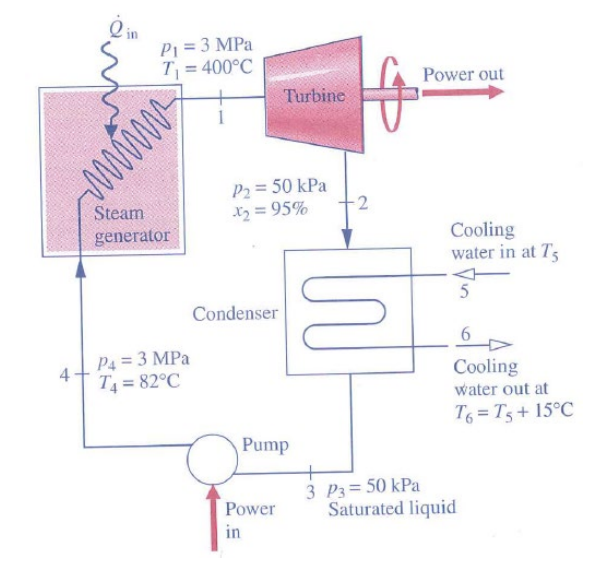
\includegraphics[width=0.8\linewidth]{hw5_q1_config.png}
    \caption{System analyzed in Question 1}
    \label{fig:q1_config}
\end{figure}

First, to find the thermal efficiency. This is simply the net work divided by the heat in:
\begin{equation}
    \eta_{th} = \frac{\Dot{W}_{Turb} - \Dot{W}_{Pump}}{\Dot{Q}_{S.G.}}
    \label{hw5:etaq1}
\end{equation}

To find $\Dot{W}_{Turb}$, we multiply the mass flow rate at the inlet and outlet by their respective enthalpies, and subtract the outlet from the inlet; however because the flow rates are the same we can factor this out like so:

\begin{equation}
    \Dot{W}_{Turb} = \Dot{m}_i \cdot \left( h_1 - h_2\right)
\end{equation}

where the $i$ subscript denotes 'inside' for the main loop; whereas 'o' would denote the cooling water loop.

Further, for the pump, this time the inlet is subtracted from the outlet:

\begin{equation}
    \Dot{W}_{Pump} = \Dot{m}_i \cdot \left( h_4 - h_3\right)
\end{equation}

Finally, the heat generation term is simply outlet minus inlet:

\begin{equation}
    \Dot{Q}_{S.G.} = \Dot{m}_i \cdot \left( h_1 - h_4\right)
\end{equation}

Finding all material properties (enthalpies) with pyXSteam, and inserting these previous equations into Eq. \ref{hw5:etaq1}, we notice the mass flow rate cancels out:

\[
    \boxed{\eta_{th} = \frac{(h_1 - h_2) - (h_4 - h_3)}{(h_1 - h_4)} = 0.24131 = 24.131\%}
\]

Next, to solve for the mass flow ratio. First we define our control volume to be over the condenser, and then begin with our conservation of energy equation.

\begin{equation}
    \label{hw5:cons_ener}
    \frac{\partial}{\partial t} \int_{CV} (\rho e) dV = \sum \Dot{Q} - \sum \Dot{W} + \sum_{i} \Dot{m}_j \left( h_j + \frac{v_j^2}{2} + gz_j \right)
\end{equation}

Next, because the problem is steady state, we can cancel out the time derivative and integral, then because there is no heating or external work done the $\Dot{Q}$ and $\Dot{W}$ summation go to 0. Thus we are left with only:

\begin{equation}
    0 = \Dot{m}_i (h_2 - h_3) + \Dot{m}_o (h_5 - h_6)
\end{equation}

and rearranging, then substituting in our determined values for enthalpy:
\[
    \boxed{\frac{\Dot{m}_o}{\Dot{m}_i} = - \frac{h_2 - h_3}{h_5 - h_6} = 34.9104}
\]

\newpage

\section*{Question 2}
\addcontentsline{toc}{section}{\protect\numberline{}Question 2}

To begin, we calculate the thermal efficiency for each cycle. The following equations are utilized, with the subscript denoting which cycle. Again all enthalpies were found using pyXSteam.

\subsection*{Part A}
\addcontentsline{toc}{subsection}{\protect\numberline{}Part A}

\[
    \boxed{\eta_{th,1} = \frac{(h_1 - h_2) - (h_{3'} - h_3)}{(h_1 - h_{3'})} = 0.38178 = 38.178\%}
\]

\[
    \boxed{\eta_{th,2} = \frac{(h_1 - h_2) - (h_{4} - h_3)}{(h_1 - h_{4})} = 0.45924 = 45.924\%}
\]
    
\[
    \boxed{\eta_{th,3} = \frac{(h_1 - h_2) - (h_{3'} - h_3)}{(h_1 - h_{3p})} = 0.36842 = 36.842\%}
\]

And then for each steam generation rate:

\[
\boxed{S.R._1 = \frac{1}{(h_1 - h_2) - (h_{3'} - h_3)} = 3.60475 \frac{kg}{kWe \cdot hr}}
\]

\[
\boxed{S.R._2 = \frac{1}{(h_1 - h_2) - (h_{4} - h_3)} = 5.38439 \frac{kg}{kWe \cdot hr}}
\]

\[
\boxed{S.R._3 = \frac{1}{(h_1 - h_2) - (h_{3'} - h_3)} = 3.54076 \frac{kg}{kWe \cdot hr}}
\]

\subsection*{Part B}
\addcontentsline{toc}{subsection}{\protect\numberline{}Part B}
The Carnot efficiency is defined as (temperatures are in kelvin):

\begin{equation}
    \eta_c = 1 - \frac{T_c}{T_h} = 0.45924 = 45.924 \%
\end{equation}

Thus, investigating all three thermal efficiencies, we determine that the second cycle is the closest to the carnot efficiency, and is thus the closest to optimal of the three cycles. 

\subsection*{Part C}
\addcontentsline{toc}{subsection}{\protect\numberline{}Part C}
To begin, all enthalpy values are in units $\frac{kj}{kg}$.

First, Cycle 1. The amount of heat added from $4\rightarrow1$ is 1455.871821738478, and from $3'\rightarrow4$ is 1160.0085423929545.

Second, Cycle 2. The amount of heat added from $4\rightarrow1$ is 1455.871821738478 again, and from $3'\rightarrow4$ is 337.866766773578. 

Finally, Cycle 3. The amount of heat added from $4\rightarrow1$ is 1596.9248939126, and from $3'\rightarrow4$ is 1162.7879446482546. 

\subsection*{Part D}
\addcontentsline{toc}{subsection}{\protect\numberline{}Part D}
To begin with, I would utilize Cycle 1. I would utilize this cycle because it has the highest thermal efficiency / steam rate --- such that the pump is operating with single-phase flow. In an ideal world, cycle two would be the strongest candidate but utilizing a pump with two-phase flow requires much more input work. However, the work output from the turbine is much higher in cycle 3, as the steam is super-heated. Also, cycle 3 has the highest power output of the 3 cycles, with cycle 2 being the lowest. 


\newpage
\section*{Question 3}
\addcontentsline{toc}{section}{\protect\numberline{}Question 3}

To begin, Fig. \ref{fig:q3_config} contains the system we are investigating.

\begin{figure}[!h!]
    \centering
    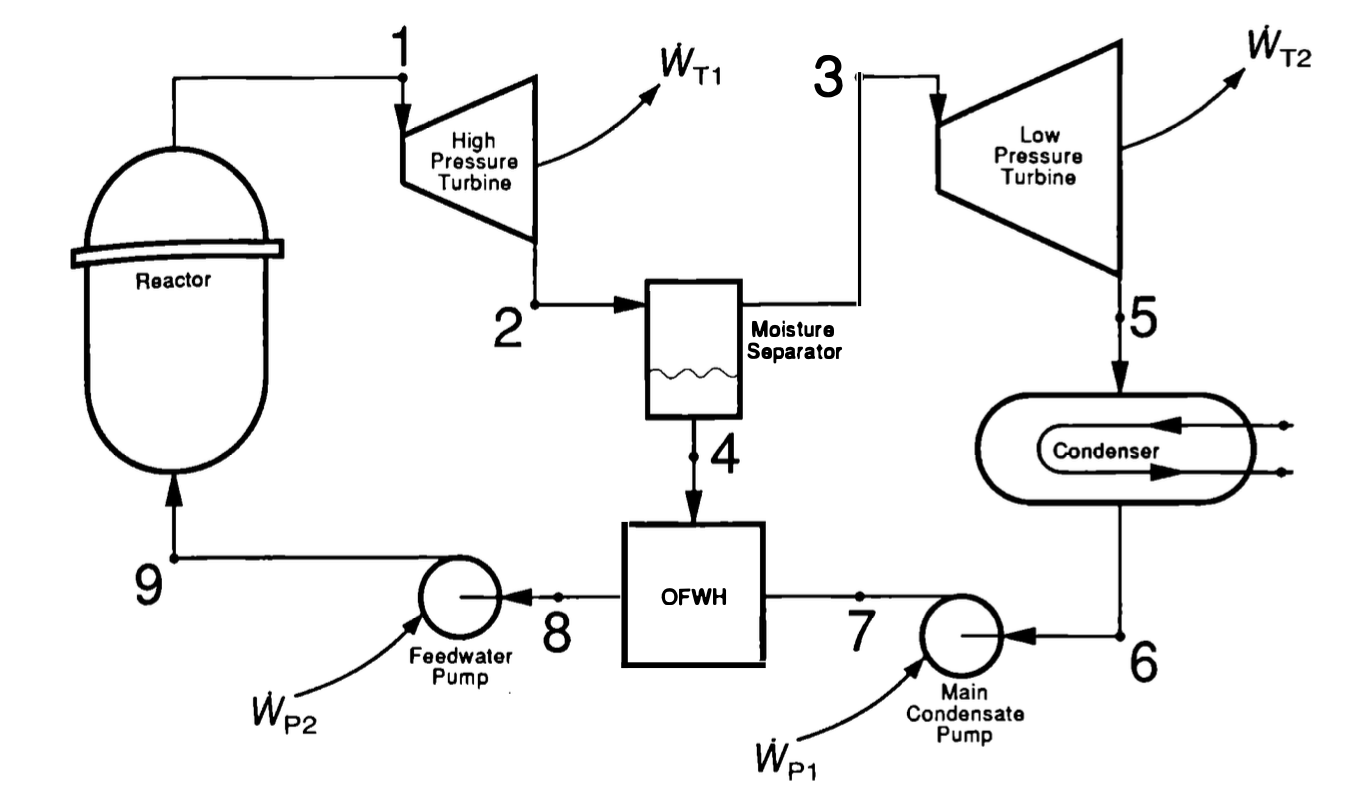
\includegraphics[width=0.8\linewidth]{hw5_q3_config.png}
    \caption{Question 3 system}
    \label{fig:q3_config}
\end{figure}

First, to find the cycle thermal efficiency. First, the equation for the thermal efficiency:

\begin{equation}
    \eta_{th} = \frac{\Dot{W}_{T,1} + \Dot{W}_{T,2} - \Dot{W}_{P,1} - \Dot{W}_{P,1}}{\Dot{Q}_R}
\end{equation}

next, our individual equations, such that subscript 'prim' and 'sec' are for the primary and secondary loops, and subscript 's' and 'r' are for enthalpies from isentropic processes and their respective real enthalpies. 

\begin{equation}
    \Dot{W}_{T,1} = \eta_{turb} \cdot (h_1 - h_{2s}) 
\end{equation}

\begin{equation}
    \Dot{W}_{T,2} = \eta_{turb} \cdot (h_3 - h_{5s}) 
\end{equation}

\begin{equation}
    \Dot{W}_{P,1} = \frac{\cdot (h_{7s} - h_{6})}{\eta_{pump}} 
\end{equation}

\begin{equation}
    \Dot{W}_{P,2} = \frac{\cdot (h_{9s} - h_{6})}{\eta_{pump}} 
\end{equation}

\begin{equation}
    \Dot{Q}_{R} = h1 - h_{9r}
\end{equation}

the first three of these equations can be instantly solved with the information available to us. However, we must find $h_8$ and $h_9$. To do this we impose a control volume around the moisture seperator. With this CV, we then investigate the conservation of mass. 

\begin{equation}
    \frac{\partial}{\partial t} \int_{CV} (\rho) dV = \sum_j \Dot{m}_j
\end{equation}

Initially, the partial derivative is ignored because it is steady state. Next, by recognizing that node 2 is two-phase flow, and node 3 and 4 are both saturated vapor /liquid single phase, we can then deduce the following relationship between mass flow rates:

\begin{equation}
    \Dot{m}_2 = \chi_2 \Dot{m}_1
\end{equation}

and 

\begin{equation}
    \Dot{m}_i = (1 - \chi_2) \Dot{m}_1
\end{equation}

And then investigating the heater as a CV and then with the conservation of energy (Eq. \ref{hw5:cons_ener}), making the same assumptions from earlier: 

\begin{equation}
    0 = \Dot{m}_1 h_8 - \Dot{m}_i h_4 - \Dot{m}_2 h_{7r}
\end{equation}

Rearranging and substituting in properties:

\begin{equation}
    h_8 = (1-\chi_2) h_4 + \chi_2 (h_6 - \Dot{W}_{P,1}) 
\end{equation}

And then, from $h_8$ we can determine $h_{9r}$ (and $h_{9s}$ from a table lookup):

\begin{equation}
    h_{9r} = h_8 - \Dot{W}_{P,2} 
\end{equation}

Finally, we have all of the information required to calculate all of the works and heat rates! Thus:

\[
    \boxed{\eta_{th} = \frac{\Dot{W}_{T,1} + \Dot{W}_{T,2} - \Dot{W}_{P,1} - \Dot{W}_{P,1}}{\Dot{Q}_R} = 0.33912 = 33.912\%}
\]

Redoing the calculation but replacing every mechanical efficiency with 100\%:

\[
\boxed{\eta_{th} = 0.37470 = 37.470\%}
\]
\newpage
\section*{Python Code}
\addcontentsline{toc}{section}{\protect\numberline{}Python Code}

\subsection*{General Code}\label{sec:gen_code}
\addcontentsline{toc}{subsection}{\protect\numberline{}General Code}


\begin{python}
    import numpy as np 
    import numpy.linalg as la
    import pandas as pd
    from pyXSteam.XSteam import XSteam as xs
    props = xs(xs.UNIT_SYSTEM_BARE) #set units to m/kg/sec/K/MPa/W

    '''
    Basic Definitions
    '''
    def wT(hin,houts,eta):
        return eta*(hin-houts)
    
    def wP(hin,houts,eta):
        return (hin-houts)/eta
\end{python}

\subsection*{Question 1}\label{sec:q1code}
\addcontentsline{toc}{subsection}{\protect\numberline{}Question 1}

\begin{python}
    '''
    Getting Material Properties
    '''
    t1,t5,t4 = np.array([400,20,82])+273.15
    h1 = props.h_pt(3,t1)
    h2 = props.h_px(.05,.95)
    h3 = props.hL_p(.05)
    h4 = props.h_pt(3,t4)
    h5 = props.h_pt(0.101325,t5)
    h6 = props.h_pt(0.101325,t5+15)
    
    '''
    Getting work / q
    '''
    wt = h1-h2
    wp = h4-h3
    qsg = h1-h4
    
    eta = (wt-wp)/qsg
    mdot_ratio = -(h2-h3)/(h5-h6)
\end{python}

\subsection*{Question 2}\label{sec:q2code}
\addcontentsline{toc}{subsection}{\protect\numberline{}Question 2}

\begin{python}
    thigh,tlow = 293+273.15,33+273.15
    '''
    Getting Material Properties
    '''
    #First cycle
    
    c1_h1 = props.hV_t(thigh)
    c1_p1 = props.psat_t(thigh)
    c1_h2 = props.h_ps(props.psat_t(tlow),props.sV_t(thigh))
    c1_h3 = props.hL_t(tlow)
    c1_h3p = props.h_ps(c1_p1,props.sL_t(tlow))
    c1_h4 = props.hL_t(thigh)
    
    c1_eta = np.around(((c1_h1-c1_h2)-(c1_h3p-c1_h3))/(c1_h1-c1_h3p),5)
    c1_steam = np.around(3600/((c1_h1-c1_h2)-(c1_h3p-c1_h3)),5)
    
    #Second Cycle
    
    c2_h1 = props.hV_t(thigh)
    c2_h2 = props.h_ps(props.psat_t(tlow),props.sV_t(thigh))
    c2_h4 = props.hL_t(thigh)
    c2_h3 = props.h_ps(props.psat_t(tlow), props.sL_t(thigh))
    
    c2_eta = np.around(((c2_h1-c2_h2)-(c2_h4-c2_h3))/(c2_h1-c2_h4),5)
    c2_steam = np.around(3600 / ((c2_h1-c2_h2)-(c2_h4-c2_h3)),5)
    
    #Third Cycle
    
    c3_h1 = props.h_pt(5,thigh)
    c3_h2 = props.h_ps(props.psat_t(tlow),props.s_pt(5,thigh))
    c3_h3 = props.hL_t(tlow)
    c3_h3p = props.h_ps(5,props.sL_t(tlow))
    c3_h4 = props.hL_t(thigh)
    c3_h5 = props.hV_t(thigh)
    
    c3_eta = np.around(((c3_h1-c3_h2) - (c3_h3p-c3_h3))/(c3_h1-c3_h3p),5)
    c3_steam = np.around(3600 / ((c3_h1-c3_h2) - (c3_h3p-c3_h3)),5)
    
\end{python}

\newpage
\subsection*{Question 3}\label{sec:q3code}
\addcontentsline{toc}{subsection}{\protect\numberline{}Question 3}

\begin{python}
    '''Getting Basic enthalpies'''
    etat,etap = .9,.85
    h1 = props.hV_p(6.890)
    h2 = props.h_ps(1.380,props.sV_p(6.890))
    h3 = props.hV_p(1.380)
    h4 = props.hL_p(1.380)
    h5 = props.h_ps(6.89/1000,props.sV_p(1.380))
    h6 = props.hL_p(6.89/1000)
    h7 = props.h_ps(1.380,props.sL_p(6.89/1000))
    
    '''Getting Basic Works'''
    wt1 = wT(h1,h2,etat)
    wt2 = wT(h3,h5,etat)
    wp1 = wP(h7,h6,etap)
    
    '''
    Geting relationship between mass flow rates of
    primary / secondary / intermediate loops:
    
    m1 = mass flow rate at left loop 
    m2 = mass flow rate at right loop 
    mi = mass flow rate at intermediate loop 
    x2 = steam quality @ node 2
    m2 = m1*x2
    mi = m1*(1-x2)
    '''
    x2 = props.x_ph(1.380,h1-wt1) #adjusting for h2 from h2s
    h8 = (1-x2)*h4 + x2*(h6-wp1) #adjusting for h7 from h7s, (mi*h4 + m2*h7) / m1 --- CV over OFWH 
    s8 = props.s_ph(1.380,h8)
    h9 = props.h_ps(6.89,s8)
    
    '''Final work / Q'''
    wp2 = wP(h9,h8,etap)
    qr = h1-(h8-wp2) #adjust for h9 from h9s
    
    '''Output'''
    therm_efficiency = (wt1+x2*wt2-x2*wp1-wp2)/(qr) #change m2 to x2*m1, cancel out m1
\end{python}

\end{document}